The three main pillars of robotic autonomy can broadly be characterized as perception, planning, and control (i.e. the ``see, think, act'' cycle). Perception categorizes those challenges associated with a robot sensing and understanding its environment, which are addressed by using various sensors and then extracting meaningful information from their measurements. The next few chapters will focus on the perception/sensing problem in robotics, and in particular will introduce common sensors utilized in robotics, their key performance characteristics, as well as strategies for extracting useful information from the sensor outputs.

\notessection{Introduction to Robot Sensors}
\nocite{SiegwartNourbakhshEtAl2011}
Robots operate in diverse environments and often require diverse sets of sensors to appropriately characterize them. For example, a self-driving car may utilize cameras, stereo cameras, lidar, and radar. Additionally, sensors are also required for characterizing the physical state of the vehicle itself, for example wheel encoders, heading sensors, GNSS positioning sensors\footnote{Global Navigation Satellite System}, and more\cite[\baselineskip]{SiegwartNourbakhshEtAl2011}. 

\subsection{Sensor Classifications}
To distinguish between sensors that measure the environment and sensors that measure quantities related the robot itself, sensors are categorized as either \textit{proprioceptive} or \textit{exteroceptive}.
\begin{definition}[Proprioceptive]
Proprioceptive sensors measure values internal to the robot, for example motor speed, wheel load, robot arm joint angles, and battery voltage.
\end{definition}

\begin{definition}[Exteroceptive]
Exteroceptive sensors acquire information from the robot’s environment, for example distance measurements, light intensity, and sound amplitude. 
\end{definition}
Generally speaking, exteroceptive sensor measurements are often more likely to require interpretation by the robot in order to extract meaningful environmental features.
In addition to characterizing \textit{what} the sensor measures, it is also useful to characterize sensors based on \textit{how} they operate. In particular it is common to characterize a sensor as either \textit{passive} or \textit{active}.
\begin{definition}[Passive Sensor]
Passive sensors measure ambient environmental energy entering the sensor, for example thermometers and cameras.
\end{definition}
\begin{definition}[Active Sensor]
Active sensors emit energy into the environment and measure the reaction, for example ultrasonic sensors and laser rangefinders. 
\end{definition}
Classifying a sensor as active or passive is important because this property introduces unique challenges. For example the performance of passive sensors depend heavily on the environment, such as a camera being dependent on the ambient lighting to get a good image.


\subsection{Sensor Performance}
Different types sensors also have different types of performance characteristics. Some sensors provide extreme accuracy in well-controlled laboratory settings but are overcome with error when subjected to real-world environmental variations. Other sensors provide narrow, high-precision data in a wide variety of settings. In order to quantify and compare such performance characteristics it is necessary to define relevant metrics. These metrics are generally either related to \textit{design specifications} or \textit{in situ} performance (i.e. how well a sensor performs in the real environment). 

\subsubsection{Design Specification Metrics} 
A number of performance characteristics are specifically considered when designing the sensor, and are also used to quantify its overall nominal performance capabilities.

\begin{enumerate}
    \item \textit{Dynamic range} quantifies the ratio between the lower and upper limits of the sensor inputs under normal operation. This metric is usually expressed in decibels (dB), which is computed as
    \begin{equation*}
        \text{DR} = 10 \log_{10}(r) \:\:[\text{dB}],
    \end{equation*}
    where $r$ is the ratio between the upper and lower limits. In addition to dynamic range (ratio), the actual range is also an important sensor metric. For example, an optical rangefinder will have a minimum operating range and can thus provide spurious data when measurements are taken with the object closer than that minimum.
    \item \textit{Resolution} is the minimum difference between two values that can be detected by a sensor. Usually, the lower limit of the dynamic range of a sensor is equal to its resolution. However, this is not necessarily the case for digital sensors.
    \item \textit{Linearity} characterizes whether or not the sensor's output depends linearly on the input.
    \item \textit{Bandwidth} or \textit{frequency} is used to measure the speed with which a sensor can provide a stream of readings. This metric is usually expressed in units of Hertz (Hz), which is measurements per second. High bandwidth sensors are usually desired so that information can be updated at a higher rate. For example, mobile robots may have a limit on their maximum speed based on the bandwidth of their obstacle detection sensors.
\end{enumerate}



\subsubsection{In Situ Performance Metrics} 
Metrics related to the design specifications can be reasonably quantified in a laboratory environment and then extrapolated to predict performance during real-world deployment. However, a number of important sensor metrics cannot be adequately characterized in laboratories settings since they are influenced by complex interactions between the environment. 

\begin{enumerate}
    \item \textit{Sensitivity} defines the ratio of change in the output from the sensor to a change in the input. High sensitivity is often undesirable because any noise to the input can be amplified, but low sensitivity might degrade the ability to extract useful information from the sensor's measurements.
    \textit{Cross-sensitivity} defines the sensitivity to environmental parameters that are unrelated to the sensor's target quantity. For example, a flux-gate compass can demonstrate high sensitivity to magnetic north and is therefore useful for mobile robot navigation. However, the compass also has high sensitivity to ferrous building materials, so much so that its cross-sensitivity often makes the sensor useless in some indoor environments. High cross-sensitivity of a sensor is generally undesirable, especially when it cannot be modeled.
    \item \textit{Error} of a sensor is defined as the difference between the sensor’s output measurements and the true values being measured, within some specific operating context. Given a true value $v$ and a measured value $m$, the error is defined as $e:=m-v$.
    \item \textit{Accuracy} is defined as the degree of conformity between the sensor’s measurement and the true value, and is often expressed as a proportion of the true value (e.g., 97.5\% accuracy). Thus small error corresponds to high accuracy and vice versa. For a measurement $m$ and true value $v$, the accuracy is defined as $a:=1-|m-v|/v$. 
    Since obtaining the true value $v$ can be difficult or impossible, characterizing sensor accuracy can be challenging.
    \item \textit{Precision} defines the reproducibility of the sensor results. For example, a sensor has high precision if multiple measurements of the same environmental quantity are similar. It is important to note that precision is not the same as accuracy, a highly precise sensor can still be highly inaccurate.
\end{enumerate}

\subsubsection{Sensor Errors}
When discussing in situ performance metrics such as accuracy and precision, it is often important to also be able to reason about the sources of sensor errors. In particular it is important to distinguish between two main types of error, \textit{systematic errors} and \textit{random errors}.

\begin{enumerate}
    \item \textit{Systematic errors} are caused by factors or processes that can in theory be modeled (i.e. they are deterministic and therefore reproducible and predictable). Calibration error is a classic source of systematic error in sensors.
    \item \textit{Random errors} cannot be predicted using a sophisticated model (i.e. they are stochastic and unpredictable). Hue instability in a color camera, spurious rangefinding errors, and black level noise in a camera are all examples of random errors.
\end{enumerate}

In order to reliably use a sensor in practice it is useful to have a characterization of the systematic and random errors, which could allow for corrections to make the sensor more accurate and provide information about its precision. Quantifying the sensor error and identifying sources of error is referred to as \textit{error analysis}. Error analysis for a typical sensor might involve identifying all of the sources of systematic errors, modeling random errors (e.g. by Gaussian distributions), and then propagating the errors from each identified source to determine the overall impact on the sensor output.

Unfortunately, it is typically challenging to perform a complete error analysis in practice for several reasons. One of the main reasons is due to a \textit{blurring} between systematic and random errors that is the result of changes to the operating environment. For example, exteroceptive sensors on a mobile robot will have constantly changing measurement sources as the robot moves through the environment, and could even be influenced by the motion of the robot itself. Therefore, an exteroceptive sensor's error profile may be heavily dependent on the particular environment and even the particular state of the robot! As a more concrete example, active ranging sensors tend to have failure modes that are triggered largely by specific relative positions of the sensor and environment targets. For example, when oriented at specific angles to a smooth sheetrock wall a sonar sensor will produce specular reflections that result in highly inaccurate range measurements. During the motion of a robot, these particular relative angles would likely occur at stochastic intervals and therefore this error source might be considered \textit{random}. Yet, if the robot were to stop at the specific angle for inducing specular reflections, the error would be persistent and could be modeled as a systematic error. In summary, while systematic and random sensor errors might be well defined in controlled settings, in practical settings characterizing error becomes a lot more challenging due to the complexity and quantity of potential error sources.

\subsubsection{Modeling Uncertainty}
If all sensor measurement errors were systematic and could be modeled then theoretically they could be corrected for. However in practice this is not the case and therefore some alternative representation of the sensor error is needed. In particular, characterizing uncertainty due to random errors is typically accomplished by using \textit{probability distributions}.

Since it is effectively impossible to know all of the sources of random error for a sensor it is common to make assumptions about what the distribution of the sensor error looks like. For example, it is commonly assumed that random errors are zero-mean and symmetric, or to go slightly further that they are Gaussian. More broadly, it is commonly assumed that the distribution is \textit{unimodal}. These assumptions are usually made because they simplify the mathematical tools used for performing theoretical analyses. 

However, it is also crucial to understand the limitations of these assumptions. In fact, in many cases even the most broad assumptions (e.g. that the distribution is unimodal) can be quite wrong in practice.
As an example consider the sonar sensor once again. When ranging an object that reflects the sound signal well, the sonar will exhibit high accuracy and the random errors will generally be based on noise (e.g. from the timing circuitry). In this operating instance it might be a perfectly fine assumption that the noise distribution is unimodal and perhaps even Gaussian. However, if the sonar sensor is moving through an environment and is faced with materials that cause coherent reflection (rather than directly returning the sound signal to the sonar sensor) then overestimates of the distance to the object are likely. In this case, the error will be
biased toward positive measurement error and will be far from the correct value. Therefore it can be seen that modeling the sonar sensor uncertainty over \textit{all} operating regimes of the robot would at least require a bimodal distribution in this case. Additionally, since overestimation is more common than underestimation, the distribution should also be asymmetric.
As a second example, consider ranging via stereo vision. Once again, at least two modes of operation can be identified. If the stereo vision system correctly correlates two images, then the resulting random error will be caused by camera noise and will limit the measurement accuracy. But the stereo vision system can also correlate two images incorrectly. In such a case stereo vision will exhibit gross measurement error, and one can easily imagine such behavior violating both the unimodal and the symmetric assumptions.

\subsection{Common Sensors on Mobile Robots}
\subsubsection{Encoders} 
Encoders are electro-mechanical devices that convert motion into a sequence of digital pulses, which can then be converted to relative or absolute position measurements. These sensors are commonly used for wheel/motor sensing to determine rotation angle and rotation rate.
Since these sensors have vast applications outside of mobile robotics there has been substantial development in low-cost encoders that offer excellent resolution. In mobile robotics, encoders are one of the most popular means to control the position or speed of wheels and other motor-driven joints. These sensors are proprioceptive and therefore their estimates are expressed in the reference frame of the robot.

\begin{figure}[ht]
\centering
        \includegraphics[width=.9\textwidth]{tex/figs/ch07_figs/wheel_encoder.png}
        \caption{Quadrature optical wheel encoder. (Figure from Siegwart et al.) \nocite{SiegwartNourbakhshEtAl2011}}
        \label{fig:encoder}
\end{figure}
Optical encoders shine light onto a photodiode through slits in a metal or glass disc, and measure the sine or square wave pulses that result from disk rotation (see Figure \ref{fig:encoder}). After some signal processing it is possible to integrate the number of wave peaks to determine how much the disk has rotated.
Encoder resolution is measured in cycles per revolution (CPR) and the minimum angular resolution can be readily computed from an encoder’s CPR rating. A typical encoder in mobile robotics may have 2000 CPR, while the optical encoder industry can readily manufacture encoders with 10,000 CPR. In terms of bandwidth, it is of course critical that the encoder is sufficiently fast to handle the expected shaft rotation rates. Luckily, industrial optical encoders present no bandwidth limitation to mobile robot applications.
Usually in mobile robotics the quadrature encoder is used. In this case, a second illumination and detector pair is placed 90 degrees shifted with respect to the original in terms of the rotor disc. The resulting twin square waves, shown in Figure \ref{fig:encoder}, provide significantly more information. The ordering of which square wave produces a rising edge first identifies the direction of rotation. Furthermore, the resolution is improved by a factor of four with no change to the rotor disc. Thus, a 2000 CPR encoder in quadrature yields 8000 counts.

As with most proprioceptive sensors, encoders typically operate in a very predictable and controlled environment. Therefore systematic errors and cross-sensitivities can be accounted for. In practice, the accuracy of optical encoders is often assumed to be 100\% since any encoder errors are dwarfed by errors in downstream components.

\subsubsection{Heading Sensors}
Heading sensors can be proprioceptive (e.g. gyroscopes, inclinometers) or exteroceptive (e.g. compasses). They are used to determine the robot’s orientation in space. Additionally, they can also be used to obtain position estimates by fusing the orientation and velocity information and integrating, a process known as \textit{dead reckoning}.

\paragraph{Compasses:} Compasses are exteroceptive sensors that measure the earth's magnetic field to provide a rough estimate of direction. In mobile robotics, digital compasses using the Hall effect are popular and they are inexpensive but often suffer from poor resolution and accuracy. Flux gate compasses have improved resolution and accuracy, but are more expensive and physically larger. Both compass types are vulnerable to vibrations and disturbances in the magnetic field, and are therefore less well suited for indoor applications.

\paragraph{Gyroscopes:} Gyroscopes are heading sensors that preserve their orientation with respect to a fixed \textit{inertial} reference frame. Gyroscopes can be classified in two categories: \textit{mechanical gyroscopes} and \textit{optical gyroscopes}.
\begin{figure}[ht]
\centering
        \includegraphics[width=.7\textwidth]{tex/figs/ch07_figs/gyro.png}
        \caption{Two-axis mechanical gyroscope. (Figure from Siegwart et al.) \nocite{SiegwartNourbakhshEtAl2011}}
        \label{fig:gyro}
\end{figure}
Mechanical gyroscopes rely on the angular momentum of a fast-spinning rotor to keep the axis of rotation inertially stable. Generally the inertial stability increases with the spinning speed $\omega$, the precession speed $\Omega$, and the wheel’s inertia $I$ since the reactive torque $\tau$ can be expressed as:
\begin{equation*}
    \tau = I \omega \Omega.
\end{equation*}
Mechanical gyroscopes are configured with an inner and outer gimbal as seen in Figure \ref{fig:gyro} such that no torque can be transmitted from the outer pivot to the wheel axis. This means that the spinning axis will therefore be space-stable (i.e. fixed in an inertial reference frame). Nevertheless, friction in the bearings of the gimbals may introduce small torques, which over time introduces small errors. A high quality mechanical gyroscope can cost up to \$100,000
and has an angular drift of about 0.1 degrees in 6 hours.

Optical gyroscopes are a relatively new invention. They use angular speed sensors with two monochromatic light beams, or lasers, emitted from the same source. Two beams are sent, one clockwise and the other counterclockwise, through an optical fiber. Since the laser traveling in the direction of rotation has a slightly shorter path, it will have a higher frequency. This frequency difference $\delta f$ is proportional to the angular velocity, which can therefore be estimated. In modern optical gyroscopes, bandwidth can easily exceed 100 kHz, while resolution can be smaller than 0.0001 degrees/hr.

\subsubsection{Accelerometer}
An accelerometer is a device used to measure net accelerations (i.e. the net external forces acting on the sensor, including gravity). Mechanical accelerometers are essentially spring-mass-damper systems that can be represented by the second order differential equation\cite{DudekJenkin2008}:
\begin{equation*}
F_{\text{applied}} = m \ddot{x} + c \dot{x} + k x
\end{equation*}
where $m$ is the proof mass, $c$ is the damping coefficient, $k$ is the spring constant, and $x$ is the relative position to a reference equilibrium. When a static force is applied, the system will oscillate until it reaches a steady state where the steady state acceleration would be given as:
\begin{equation*}
    a_{applied} = \frac{kx}{m}.
\end{equation*}
The design of the sensor chooses $m$, $c$, and $k$ such that system can stabilize quickly and then the applied acceleration can be calculated from steady state.
Modern accelerometers, such as the ones in mobile phones, are usually very small and use Micro Electro-Mechanical Systems (MEMS), which consist of a cantilevered beam and a proof mass. The deflection of the proof mass from its neutral position is measured using capacitive or piezoelectric effects.


\subsubsection{Inertial Measurement Unit (IMU)}
Inertial measurement units (IMU) are devices that use gyroscopes and accelerometers to estimate their relative position, orientation, velocity, and acceleration with respect to an inertial reference frame. Their general working principle is shown in Figure \ref{fig:IMU}.

The gyroscope data is integrated to estimate the vehicle orientation while the three accelerometers are used to estimate the instantaneous acceleration of the vehicle. The acceleration is then transformed to the local navigation frame by means of the current estimate of the vehicle orientation relative to gravity. At this point the gravity vector can be subtracted from the measurement. The resulting acceleration is then integrated to obtain the velocity and then integrated again to obtain the position, provided that both the initial velocity and position are a priori known. 
To overcome the need of knowing of the initial velocity, the integration is typically started at rest when the velocity is zero.

One of the fundamental issues with IMUs is the phenomenon called \textit{drift}, which describes the slow accumulation of errors over time. Drift in any one component will also effect the downstream components as well. For example, drift in the gyroscope unavoidably undermines the estimation of the vehicle orientation relative to gravity, which results in incorrect cancellation of the gravity vector. Additionally, errors in acceleration measurements will cause the integrated velocity to drift in time (which will in turn also cause position estimate drift). To account for drift periodic references to some external measurement is required. In many robot applications, such an external reference may come from GNSS position measurements, cameras, or other sensors.

\begin{figure*}[ht]
    \centering
        \includegraphics[width=0.7\textwidth]{tex/figs/ch07_figs/imu.png}
      \caption{Inertial measurement unit (IMU) block diagram.}
    \label{fig:IMU}
\end{figure*}

\subsubsection{Beacons}
Beacons are signaling devices with precisely known positions (e.g. stars and lighthouses are classic examples). Position of a mobile robot can be determined by knowing the position of the beacon and by having access to relative position measurements. The GNSS positioning system and camera-based motion capture system for indoor use are more advanced examples. GNSS based positioning is extremely popular in robotics, and works by processing synchronized signals from at least four satellites. Signals from four satellites are needed (at a minimum) to enable the estimation of four unknown quantities (the three position coordinates plus a clock correction). Modified GNSS-based methods, such as differential GPS, can be used to increase positioning accuracy.

\subsubsection{Active Ranging}
Active ranging sensors provide direct measurements of distance to objects in the vicinity of the sensor. These sensors are important in robotics for both localization and environment reconstruction. There are two main types of active ranging sensors: time-of-flight active ranging sensors (e.g. ultrasonic, laser rangefinder, and time-of-flight cameras) and geometric active ranging sensors (e.g. based on optical triangulation and structured light).

\begin{marginfigure}
\centering
\includegraphics[scale=0.8]{tex/figs/ch07_figs/Velodyne_64e.png}
\caption{The Velodyne HDL-64E High Definition Real-Time 3D Lidar sensor, a time-of-flight active ranging sensor. (Image retrieved from velodynelidar.com)}
\label{fig:active_range}
\end{marginfigure}

\paragraph{Time-of-flight Active Ranging:} 
Time-of-flight active ranging sensors make use of the propagation speed of sounds or electromagnetic waves. In particular, the travel distance is given by 
\begin{equation*}
    d = c t,
\end{equation*} 
where $d$ is the distance traveled, $c$ is the speed of wave propagation, and $t$ is the time of flight. The propagation speed $c$ of sound is approximately $0.3 m/ms$ whereas the speed of electromagnetic signals is $0.3 m/ns$, which is 1 million times faster! The time of flight for a distance of $3$ meters is $10$ milliseconds for an ultrasonic system, but only $10$ nanoseconds for a laser rangefinder, which makes measuring the time of flight $t$ for electromagnetic signals more technologically challenging. This explains why laser range sensors have only recently become affordable and robust for use on mobile robots.
The quality of different time-of-flight range sensors may depend on:
\begin{enumerate}
    \item uncertainties in determining the exact time of arrival of the reflected signal,
    \item inaccuracies in the time-of-flight measurement (particularly with laser range sensors),
    \item the dispersal cone of the transmitted beam (mainly with ultrasonic range sensors),
    \item interaction with the target (e.g. surface absorption, specular reflections),
    \item variation of propagation speed,
    \item the speed of the mobile robot and target (in the case of a dynamic target).
\end{enumerate}


\paragraph{Geometric Active Ranging:} 
Geometric active ranging sensors use geometric properties in the measurements to establish distance readings. Generally, these sensors project a known pattern of light and then geometric properties can be used to analyze the reflection and estimate range via triangulation.
Optical triangulation sensors (1D) transmit a collimated (parallel rays of light) beam toward the target and use a lens to collect reflected light and project it onto a position-sensitive device or linear camera. Structured light sensors (2D or 3D) project a known light pattern (e.g. point, line, or texture) onto the environment. The reflection is captured by a receiver and then, together with known geometric values, range is estimated via triangulation. 

\subsubsection{Other Sensors}
Some classical examples of other sensors include radar, tactile sensors, and vision based sensors (e.g. cameras). Radar sensors leverage the Doppler effect to produce velocity relative velocity measurements. Tactile sensors are particularly useful for robots that interact physically with their environment. 

\subsection{Computer Vision}
Vision sensors have become crucial sensors for perception in the context of robotics. This is generally due to the fact that vision provides an enormous amount of information about the environment and enables rich, intelligent interaction in dynamic environments\footnote{In fact, the human eye provides millions of bits of information per second.}. The main challenges associated with vision-based sensing are related to processing digital images to extract salient information like object depth, motion and object detection, color tracking, feature detection, scene recognition, and more.
The analysis and processing of images are generally referred to as \textit{computer vision} and \textit{image processing}. Tremendous advances and new theoretical findings in these fields over the last several decades have led to sophisticated computer vision and image processing techniques to be utilized in industrial and consumer applications such as photography, defect inspection, monitoring and surveillance, video games, movies, and more. 
This section introduces some fundamental concepts related to these fields, and in particular will focus on cameras and camera models.

\subsubsection{Digital Cameras}
While the basic idea of a camera has existed for thousands of years, the first clear description of one was given by Leonardo Da Vinci in 1502 and the oldest known published drawing of a \textit{camera obscura} (a dark room with a pinhole to image a scene) was shown by Gemma Frisius in 1544. By 1685, Johann Zahn had designed the first portable camera, and in 1822 Joseph Nicephore Niepce took the first physical photograph.

Modern cameras consist of a sensor that captures light and converts the resulting signal into a digital image. Light falling on an imaging sensor is usually picked up by an active sensing area, integrated for the duration of the exposure (usually expressed as the shutter speed, e.g. $1/125, 1/60, 1/30$ of a second), and then passed to a set of sense amplifiers. The two main kinds of sensors used in digital cameras today are charge coupled devices (CCD) and complementary metal oxide on silicon (CMOS) sensors.
A CCD chip is an array of light-sensitive picture elements (pixels), and can contain between 20,000 and several million pixels total. Each pixel can be thought of as a light-sensitive discharging capacitor that is $5$ to $25\mu \text{m}$ in size. While complementary metal oxide semiconductor (CMOS) chips also consist of an array of pixels, they are quite different from CCD chips. In particular, along the side of each pixel are several transistors specific to that pixel. CCD sensors have typically outperformed CMOS for quality sensitive applications such as digital single-lens-reflex cameras, while CMOS sensors are better for low-power applications. However, today CMOS sensors are standard in most digital cameras.

\subsubsection{Image Formation}
Before reaching the camera's sensor, light rays first originate from a light source. In general the rays of light reflected by an object tend to be scattered in many directions and may consist of different wavelengths. 
Averaged over time, the emitted wavelengths and directions for a specific object can be precisely described using object-specific probability distribution functions. In particular, the light reflection properties of a given object are the result of how light is reflected, scattered, or absorbed based on the object's surface properties and the wavelength of the light. For example, an object might look blue because blue wavelengths of light are primarily scattered off the surface while other wavelengths are absorbed. Similarly, a black object looks black because it absorbs most wavelengths of light, and a perfect mirror reflects all visible wavelengths.

Cameras capture images by sensing these light rays on a photoreceptive surface (e.g. a CCD or a CMOS sensor). However, since light reflecting off an object is generally scattered in many directions, simply exposing a planar photoreceptive surface to these reflected rays would result in many rays being captured at each pixel. This would lead to blurry images! A solution to this issue is to add a barrier in front of the photoreceptive surface that blocks most of these rays, and only lets some of them pass through an aperture (see Figure \ref{fig:LightRays}). 
The earliest approach to filtering light rays in this way was to have a small hole in the barrier surface. Cameras with this type of filter were referred to as \textit{pinhole} cameras.
\begin{figure}[ht]
\centering
\includegraphics[width=0.95\textwidth]{tex/figs/ch07_figs/pinhole.png}
\caption{Light rays on a photoreceptive surface referred to as the image plane. On the left, numerous rays being reflected and scattered by the object leads to blurry images whereas (on the right), a barrier has been added so that the scattered light rays can be distinguished.}
\label{fig:LightRays}
\end{figure}


\subsubsection{Pinhole Camera Model} 
A pinhole camera has no lens but rather a single very small aperture. Light from the scene passes through this pinhole aperture and projects an inverted image onto the image plane (see Figure \ref{fig:PinholeMath}). While modern cameras do not operate in this way, the principles of the pinhole camera can be used to derive useful mathematical models. 

\begin{figure}[ht]
\centering
\includegraphics[width=0.85\textwidth]{tex/figs/ch07_figs/pinholecamera.png}
\caption{Pinhole camera model. Due to the geometry of the pinhole camera system, the object's image is inverted on the image plane. In this figure, $O$ is the camera center, $c$ is the image center, and $p$ the principal point.}
\label{fig:PinholeMath}
\end{figure}

To develop the mathematical pinhole camera model, several useful reference frames are defined. First, the \textit{camera reference frame} is centered at a point $O$ (see Figure \ref{fig:PinholeMath}) that is at a focal length $f$ in front of the image plane. This reference frame with directions $(i,j,k)$ is defined with the $k$ axis coincident with the \textit{optical axis} that points toward the image plane. The coordinates of a point in the camera frame are denoted by uppercase $P = (X,Y,Z)$. When a ray of light is emitted from a point $P$ and passes through the pinhole at point $O$, it gets captured on the image plane at a point $p$. Since these points are all collinear it is possible to deduce the following relationships between the coordinates $P = (X,Y,Z)$ and $p = (x,y,z)$:
\begin{equation*}
x = \lambda X, \quad y = \lambda Y, \quad z = \lambda Z,
\end{equation*}
for some $\lambda \in \R$. This leads to the relationship:
\begin{equation*}
\lambda = \frac{x}{X}= \frac{y}{Y}= \frac{z}{Z}.
\end{equation*}
Further, from the geometry of the camera it can be seen that $z = f$ where $f$ is the focal length, such that these expressions can be rewritten as:
\begin{equation} \label{eq:pinhole}
    x=f\frac{X}{Z}, \quad  y = f\frac{Y}{Z}.
\end{equation}
Therefore the position of the pixel on the image plane that captures a ray of light from the point $P$ can be computed.

\subsubsection{Thin Lens Model}
One of the main issues with having a fixed pinhole aperture is that there is a trade-off associated with the aperture's size. A large aperture allows a greater number of light rays to pass through, which leads to blurring of the image. However, a small aperture lets through fewer light rays and the resulting image is darker. As a solution, lenses can focus light via refraction and can be used to replace the aperture, therefore avoiding the need for these trade-offs. 

A similar mathematical model to the pinhole model can be introduced for lenses by using properties from Snell's law. Figure \ref{fig:Lens} shows a diagram of the most basic lens model, which is the \textit{thin lens model} (which assumes no optical distortion due to the curvature of the lens). Snell's law states that rays passing through the center of the lens are not refracted, and those that are parallel to the optical axis are focused on the focal point labeled $F'$. In addition, all rays passing through $P$ are focused by the thin lens on the point $p$. From the geometry of similar triangles, a mathematical model similar to \eqref{eq:pinhole} is developed:
\begin{equation}
    \frac{y}{Y}=\frac{z}{Z}, \quad \frac{y}{Y}=\frac{z-f}{f}  = \frac{z}{f} -1,
\end{equation}
where again the point $P$ has coordinates $(X,Y,Z)$, its corresponding point $p$ on the image plane has coordinates $(x,y,z)$, and $f$ is the focal length.
Combining these two equations yields the \textit{thin lens equation}:
\begin{equation} \label{eq:thinlens}
    \frac{1}{z}+\frac{1}{Z}=\frac{1}{f}.
\end{equation}
Note that in this model for a particular focal length $f$, a point $P$ is only in sharp focus if the image plane is located a distance $z$ from the lens. However, in practice an acceptable focus is possible withing some range of distances (called depth of field or depth of focus). Additionally, if $Z$ approaches infinity light would focus a distance of $f$ away from the lens. Therefore, this model is essentially the same as a pinhole model if the lens is focused at a distance of infinity.
As can be seen, this formula can also be used to estimate the distance to an object by knowing the focal length $f$ and the current distance of the image plane to the lens $z$. This technique is called \textit{depth from focus}. 

\begin{figure}[ht]
\centering
\includegraphics[width=0.8\textwidth]{tex/figs/ch07_figs/thinlens.png}
\caption{The thin lens model.}
\label{fig:Lens}
\end{figure}
